\documentclass[11pt]{article}
\usepackage[utf8]{inputenc}
\usepackage[spanish,es-tabla]{babel}
\usepackage[margin=35mm]{geometry} %Márgenes mas pequeños
\usepackage{cite}
\usepackage{amsmath,amssymb,amsfonts}
\usepackage{algorithmic}
\usepackage{graphicx}
\usepackage{textcomp}
\usepackage{xcolor}
\usepackage{booktabs}
\usepackage{optidef}
\usepackage{pdfpages}
\usepackage{float}
\usepackage{tikz}
\restylefloat{table}

\newcommand{\tikzmark}[2]{\tikz[overlay,remember picture,baseline] 
\node [anchor=base] (#1) {$#2$};}

\newcommand{\DrawVLine}[3][]{%
  \begin{tikzpicture}[overlay,remember picture]
    \draw[shorten <=0.3ex, #1] (#2.north) -- (#3.south);
  \end{tikzpicture}
}

\newcommand{\DrawHLine}[3][]{%
  \begin{tikzpicture}[overlay,remember picture]
    \draw[shorten <=0.2em, #1] (#2.west) -- (#3.east);
  \end{tikzpicture}
}

\def\BibTeX{{\rm B\kern-.05em{\sc i\kern-.025em b}\kern-.08em
    T\kern-.1667em\lower.7ex\hbox{E}\kern-.125emX}}
%Lo de arriba son como imports, no le heches cuenta ;)

\title{
        \textbf{Problema de optimización}\\
        \medskip
        \large{Trabajo de Curso}\\
        \bigskip
        Universidad de Sevilla\\ Ingeniería Informática Tecnologías Informáticas\\
        Matemática aplicada a Sistemas de Información - Tercer curso}
        
\author{
Juan Arteaga Carmona\\
Herrera, Sevilla, España \\
\texttt{JuanArteaga@andalu30.me}\\
Participación: 50\%
\and
Enrique Ramos Miró\\
Sanlúcar la Mayor, Sevilla, España \\
\texttt{kikeramos9@gmail.com}\\
Participación: 50\%
}



\begin{document}

%Portada con titulo e integrantes
\maketitle
\newpage

%Índice de la memoria
\tableofcontents
\listoftables
%\listoffigures
\newpage

%Documento----
\section{Descripción del problema general de asignación}
A continuación se muestra el ejercicio 15 del documento ``Supplementary Exercises'', el cual ha sido asignado a nuestro grupo.

\subsection{Problema asignado al grupo}\label{sec:probasig}
After qualifying, medical students must take two six-month jobs in hospital departments, but they cannot take both jobs in the same department. A hospital has four students and vacancies in four departments: Casualty, Maternity, medical and Surgical. The number of fatal mistakes each student will make in each department is given by the table \ref{tab:tablaProblema}.

\begin{table}[h!]
\centering
\begin{tabular}{@{}lcccc@{}}
\toprule
 & \multicolumn{1}{l}{Casualty} & \multicolumn{1}{l}{Maternity} & \multicolumn{1}{l}{Medical} & \multicolumn{1}{l}{Surgical} \\ \midrule
Student 1 & 3 & 0 & 2 & 6 \\
Student 2 & 2 & 1 & 4 & 5 \\
Student 3 & 4 & 2 & 5 & 7 \\
Student 4 & 2 & 0 & 2 & 4 \\ \bottomrule
\end{tabular}
%\caption{Tabla de datos del problema propuesto}
\label{tab:tablaProblema}
\end{table}

\begin{enumerate}
    \item How should they be allotted to departments for the first job so as to minimize the total mistakes?
    \item Given that allocation, how should they be allotted for the second six months so no one stays in the same job, and mistakes are minimized?
\end{enumerate}

\subsection{Problema general de asignación}
Un problema de asignación consiste en encontrar un emparejamiento de peso óptimo en un grafo bipartito ponderado, donde los pesos de las aristas se corresponden con los costes de las asignaciones, valor que se debe de minimizar.\cite{wikipediaAsignacion}. En nuestro caso nos encontramos con estudiantes que tienen que ser asignados a unos departamentos.\\

Generalmente, en los problemas de asignación a cada recurso se le asigna una única tarea, sin embargo, es posible interpretar nuestro problema de tal forma que no sea estrictamente necesario que un departamento tenga una única vacante. En este caso es posible que más de un estudiante acabe en el mismo departamento ya que han sido asignados al departamento en el que tendrán menos errores, algo más que razonable en la vida real. Por esto mismo hemos tenido en cuenta esta interpretación y también le daremos una solución.


\section{Métodos de resolución}
\subsection{El método húngaro}\label{ref:metodohungaro}
El método húngaro\cite{metodohungaroblogspot} es un método de optimización de problemas de asignación.

Este método utiliza la propiedad de reducción de matrices para reducir la matriz original de costes, hasta que los costes $C_{i,j}$ asociados con la asignación óptima, sean cero y todos los otros costes sean no negativos. En cada iteración del método húngaro, se reduce la matriz de tal manera que haya al menos un cero en cada fila y columna.

El algoritmo está diseñado para la resolución de problemas de minimización únicamente.\\\\
\textbf{Procedimiento:}\\
El Método Húngaro consta de los siguientes pasos:

\begin{itemize}
    \item \textbf{Paso 1:} En la matriz original de costo, identificar el mínimo de cada fila y restarlo de todos los elementos de la fila.
    \item \textbf{Paso 2:} En la matriz que resulte del Paso 1, identificar el mínimo de cada columna, y restarlo de todos los elementos de la columna.
    \item \textbf{Paso 3:} Identificar la solución óptima como la asignación factible asociada con los elementos cero de la matriz obtenida en el Paso 2.
\end{itemize}


\subsection{Resolución mediante SAGE}
SageMath\cite{sageweb}, comúnmente conocido por su antiguo nombre, SAGE, es un software open-source matemático creado sobre diversas librerias del lenguaje de programación Python\cite{pythonweb}.\\

Para resolver problemas de programacion lineal utilizaremos la clase \texttt{MixedIntegerLinearProgram}, que nos permite definir este tipo de problemas.\\
Definiremos las variables que aparecen en el problema con\\ \texttt{x=p.new\_variable(nonnegative=True,binary=true)}, donde es importante poner a \texttt{true} el parámetro \texttt{binary}, declararemos el objetivo con \texttt{set\_objective} y finalmente resolveremos el problema con el método \texttt{solve}\\
La solución al ejercicio propuesto con SAGE, teniendo en cuenta las dos interpretaciones, se puede ver en el Anexo 1.




\section{Resolución del problema propuesto}
\subsection{Resolución del problema considerando que no hay un mínimo de vacantes en cada departamento}

\subsubsection{Modelado mediante Programación lineal del problema propuesto}\label{ref:proglineal}
Tal y como hemos visto en el apartado \ref{sec:probasig}, los datos de nuestro problema de asignación se nos han dado en formato tabla. De esta tabla, los datos que más nos interesan son los errores que van a cometer los alumnos, que llamaremos $c$.\\
Para modelar el problema mediante programación lineal nos ayudaremos de 16 variables binarias (que llamaremos $x_{i,j}$ con $i,j = 1,..,4$) que indicarán en que departamento serán asignados los alumnos.\\

Nuestra ecuación a minimizar será $\sum{c_i x_{i,j}}$, con $i,j=1,..,4$\\
Además, necesitaremos varias restricciones para asegurarnos de obtener una solución correcta. En este caso necesitaremos de 5 restricciones, 4 para indicar que cada alumno necesita ser incluido a un único departamento y otra más para indicar que las variables son binarias.\\

De esta forma, nos quedaría el siguiente problema:\\

Sea $Z(x) = 3 x_{1,1} +0 x_{1,2} + 2 x_{1,3} + 6 x_{1,4} + 2 x_{2,1} + x_{2,2} + 4 x_{2,3} + 5 x_{2,4} + 4 x_{3,1} + 2 x_{3,2} + 5 x_{3,3} + 7 x_{3,4} + 2 x_{4,1} + 0 x_{4,2}+ 2 x_{4,3}+ 4 x_{4,4}$

\begin{mini*}
  {}{Z(x)}{}{}
  \addConstraint{x_{1,1} + x_{1,2} + x_{1,3} + x_{1,4}}{=1}{}
  \addConstraint{x_{2,1} + x_{2,2} + x_{2,3} + x_{2,4}}{=1}{}
  \addConstraint{x_{3,1} + x_{3,2} + x_{3,3} + x_{3,4}}{=1}{}
  \addConstraint{x_{4,1} + x_{4,2} + x_{4,3} + x_{4,4}}{=1}{}
  \addConstraint{x_{i,j}}{\in \{0,1\}}{\ i,j=1,..,4}
\end{mini*}

\subsubsection{Aplicación de un método de resolución para obtener el resultado al primer apartado}
Al resolver este problema de programación lineal e interpretar los resultados nos encontraremos con la solución al primer apartado del problema.

Un ejemplo de resolución se puede encontrar en el anexo 1, seccion 1.2, en el que utilizamos SAGE para resolver este problema. \label{ref:modo1SAGE}

\subsubsection{Aplicación de un método de resolución para obtener el resultado al segundo apartado}
Para solucionar el segundo apartado necesitaremos tener en cuenta los resultados del primero ya que como vimos en el apartado \ref{sec:probasig} ningún alumno puede repetir departamento. Para asegurarnos de que esto es así realizaremos algunos cambios a los costes de nuestro problema, intercambiando el valor de los costes correspondientes con las soluciones del primer apartado por $M$, un número lo suficientemente grande para que esta solución sea penalizada y, de esta forma, asegurarnos de que los alumnos no pueden repetir departamento.

La solución mediante sage se puede observar en el anexo 1, seccion 1.3.







\subsection{Resolución del problema considerando que sólo hay una vacante en cada departamento}
\subsubsection{Modelado mediante Programación lineal del problema propuesto}

El problema que nos resulta al considerar este caso es prácticamente el mismo que hemos visto en el apartado \ref{ref:proglineal}. 
Sin embargo existe una diferencia muy importante, debemos introducir varias restricciones que nos indiquen que solo existe una vacante en cada departamento.\\

De esta forma, al igual que en el caso anterior, para modelar el problema mediante programación lineal nos ayudaremos de 16 variables binarias (que llamaremos $x_{i,j}$, con $i,j=1,..,4$) que indicarán en que departamento serán asignados los alumnos.\\


Nuestra ecuación a minimizar será $\sum{c_i x_{i,j}}$ (con $i,j=1,..,4$) donde $c$ serán los errores que pueden cometer cada alumno en cada departamento y, además, tendremos las restricciones anteriores y 4 más, que nos indican que todos los departamentos reciben un alumno.\\

De esta forma, nos quedaría el siguiente problema:\\


Sea $Z(x) = 3 x_{1,1} +0 x_{1,2} + 2 x_{1,3} + 6 x_{1,4} + 2 x_{2,1} + x_{2,2} + 4 x_{2,3} + 5 x_{2,4} + 4 x_{3,1} + 2 x_{3,2} + 5 x_{3,3} + 7 x_{3,4} + 2 x_{4,1} + 0 x_{4,2}+ 2 x_{4,3}+ 4 x_{4,4}$

\begin{mini*}
  {}{Z(x)}{}{}
  \addConstraint{x_{1,1} + x_{1,2} + x_{1,3} + x_{1,4}}{=1}{}
  \addConstraint{x_{2,1} + x_{2,2} + x_{2,3} + x_{2,4}}{=1}{}
  \addConstraint{x_{3,1} + x_{3,2} + x_{3,3} + x_{3,4}}{=1}{}
  \addConstraint{x_{4,1} + x_{4,2} + x_{4,3} + x_{4,4}}{=1}{}
  \addConstraint{x_{1,1} + x_{2,1} + x_{3,1} + x_{4,1}}{=1}{}
  \addConstraint{x_{1,2} + x_{2,2} + x_{3,2} + x_{4,2}}{=1}{}
  \addConstraint{x_{1,3} + x_{2,3} + x_{3,3} + x_{4,3}}{=1}{}
  \addConstraint{x_{1,4} + x_{2,4} + x_{3,4} + x_{4,4}}{=1}{}
  \addConstraint{x_{i,j}}{\in \{0,1\}}{\ i,j=1,..,4}
\end{mini*}

\subsubsection{Aplicación de un método de resolución para obtener el resultado al primer apartado}

Al resolver este problema de programación lineal e interpretar los resultados nos encontraremos con la solución al primer apartado del problema.\\

En esta ocasión es posible resolver el problema mediante 2 métodos distintos, mediante SAGE, al igual que en el apartado \ref{ref:modo1SAGE} y con el método húngaro que se ha explicado en el apartado \ref{ref:metodohungaro}.

\begin{itemize}
    \item La resolución mediante SAGE se puede ver en el anexo 1.
    \item La resolución mediante el método húngaro se encuentra a continuación.\\
\end{itemize}


\begin{table}[H]
\centering
\begin{tabular}{lccccl}
\cline{1-5}
 & \multicolumn{1}{l}{Casualty} & \multicolumn{1}{l}{Maternity} & \multicolumn{1}{l}{Medical} & \multicolumn{1}{l}{Surgical} &  \\ \cline{1-5}
Student 1 & 3 & 0 & \textcircled{2} & 6 & 0 \\
Student 2 & \textcircled{2} & 1 & 4 & 5 & 1 \\
Student 3 & 4 & \textcircled{2} & 5 & 7 & 2 \\
Student 4 & 2 & 0 & 2 & \textcircled{4} & 0 \\ \cline{1-5}
\end{tabular}
\caption{Paso 1 del método húngaro, primer apartado}
\end{table}

En primer lugar, en el paso 1 del método húngaro vemos cuál es el número menor de cada fila, en este caso 0,1,2 y 0 para la fila 1,2,3 y 4 respectivamente. (Escrito a la derecha de la tabla).

Y a continuación se va a restar cada número por su fila (Nos damos cuenta que si es 0, se queda la fila tal cuál), es decir, por ejemplo para la fila 2 sería: 2-1 = 1, 1-1 = 0, 4-1 = 3 y 5-1 = 4. Y así sucesivamente por cada fila, donde nos quedaría finalmente la tabla 2 (justo debajo).\\

\begin{table}[H]
\centering
\begin{tabular}{lcccc}
\hline
 & \multicolumn{1}{l}{Casualty} & \multicolumn{1}{l}{Maternity} & \multicolumn{1}{l}{Medical} & \multicolumn{1}{l}{Surgical} \\ \hline
Student 1 & 3 & 0 & 2 & 6 \\
Student 2 & 1 & 0 & 3 & 4 \\
Student 3 & 3 & 0 & 3 & 5 \\
Student 4 & 2 & 0 & 2 & 4 \\ \hline
 & 1 &  & 2 & 4
\end{tabular}
\caption{Paso 2 del método húngaro, primer apartado}
\end{table}

En este paso 2 del método, hacemos lo mismo que antes en el paso 1 pero con las columnas, es decir, buscamos el número mínimo de cada columna (nos damos cuenta que si hay un 0 nos ahorramos el ponerlo porque nos quedaría igual) y se lo restamos a dicha columna. Nos queda la tabla 3 (igualmente, la que está justo debajo).\\

\begin{table}[H]
\centering
\begin{tabular}{lcccc}
\hline
 & \multicolumn{1}{l}{Casualty} & \multicolumn{1}{l}{Maternity} & \multicolumn{1}{l}{Medical} & \multicolumn{1}{l}{Surgical} \\ \hline
Student 1 &  \tikzmark{iniciolin1}{2} & \tikzmark{iniciocol2}{0} & 0 & \tikzmark{finlin1}{2} \\
Student 2 & \tikzmark{iniciolin2}{0} & 0 & 1 &  \tikzmark{finlin2}{0}\\
Student 3 & 1 & 0 & 1 & 1 \\
Student 4 & \tikzmark{iniciolin4}{1} & \tikzmark{fincol2}{0} & 0 & \tikzmark{finlin4}{0} \\ \hline
\end{tabular}
\DrawHLine[black, thick, opacity=0.8]{iniciolin1}{finlin1}
\DrawHLine[black, thick, opacity=0.8]{iniciolin2}{finlin2}
\DrawHLine[black, thick, opacity=0.8]{iniciolin4}{finlin4}
\DrawVLine[black, thick, opacity=0.8]{iniciocol2}{fincol2}
\caption{Paso 3 del método húngaro, primer apartado}
\end{table}

En este paso 3, donde nos encontremos un 0, vamos a hacer una línea para `eliminarlos'. Nos salen 4 líneas (3 horizontales y 1 vertical) y como nuestra matriz es 4x4, es decir, tenemos 4 estudiantes para 4 puestos de trabajo, habríamos acabado.\\
Donde se ubican los ceros son los lugares posibles a donde podemos enviar a cada estudiante con su correspondiente departamento.\\


\begin{itemize}
    \item \textbf{Student 1:} Maternity, Medical
    \item \textbf{Student 2:} Casualty, Maternity, Surgical
    \item \textbf{Student 3:} Maternity
    \item \textbf{Student 4:} Maternity, Medical, Surgical
\end{itemize}{}


Cómo vemos hemos asociado a cada estudiante con los ceros de la tabla y su correspondiente departamento, pues bien, al estudiante 3 ya le podríamos asignar Maternity porque sólo tiene ese 0 en esa fila, luego ya a ningún otro más se le podría asignar ese departamento así que tacharíamos Maternity de los demás estudiantes.

Y vemos que si le tachamos Maternity al estudiante 1 sólo quedaría Medical, así que le asignamos Medical al estudiante 1 e igualmente lo volveríamos a tachar si le apareciera a otro estudiante. El estudiante 4 le asignamos Surgical, el cuál sería el único, porque tanto Maternity como Medical estarían tachados. Y por último al estudiante 2 le asignamos Casualty.\\

Quedaría tal que así: 
\begin{itemize}
    \item \textbf{Student1:} Medical
    \item \textbf{Student2:} Casualty
    \item \textbf{Student3:} Maternity
    \item \textbf{Student4:} Surgical
\end{itemize}{}

Por último nos vamos a la primera tabla, 'Tabla 1' y vemos los valores de la tabla asociados a estudiante 1 y Medical, al estudiante 2 y Casualty, al estudiante 3 y Maternity y al estudiante 4 y Surgical que serían 2, 2, 2 y 4 respectivamente. Los sumamos y nos da el costo mínimo final. ($2+2+2+4 = 10$)




\subsubsection{Aplicación de un método de resolución para obtener el resultado al segundo apartado}

Para solucionar el segundo apartado necesitaremos tener en cuenta los resultados del primero ya que como vimos en el apartado \ref{sec:probasig} ningún alumno puede repetir departamento.

Una vez mas,  realizaremos algunos cambios a los costes de nuestro problema, intercambiando el valor de los costes correspondientes con las soluciones del primer apartado por $M$, un número lo suficientemente grande para que esta solución sea penalizada.

Al igual que para el primer apartado, es posible solucionarlo mediante dos métodos distintos, SAGE y el método húngaro.

\begin{itemize}
    \item La resolución mediante SAGE se puede ver, una vez mas, en el anexo 1.
    \item La resolución mediante el método húngaro se encuentra a continuación.\\
\end{itemize}

\begin{table}[H]
\centering
\begin{tabular}{lccccl}
\cline{1-5}
 & \multicolumn{1}{l}{Casualty} & \multicolumn{1}{l}{Maternity} & \multicolumn{1}{l}{Medical} & \multicolumn{1}{l}{Surgical} &  \\ \cline{1-5}
Student 1 & 3 & \textcircled{0} & M & 6 & 0 \\
Student 2 & M & 1 & 4 & \textcircled{5} & 1 \\
Student 3 & \textcircled{4} & M & 5 & 7 & 4 \\
Student 4 & 2 & 0 & \textcircled{2} & M & 0 \\ \cline{1-5}
\end{tabular}
\caption{Paso 1 del método húngaro, segundo apartado}
\end{table}

Para el segundo apartado lo que hacemos es como la resolución mediante SAGE, y es que le metemos una variable, en este caso la llamamos M, suficientemente grande donde antes nos había salido las soluciones para que penalice mucho y no vuelvan a repetirse (quedaría como la Tabla 4), por lo demás el método de resolución es el mismo que en el apartado 1, eligiendo en primer lugar el número más pequeño de cada fila y restándolo. 


\begin{table}[H]
\centering
\begin{tabular}{lcccc}
\hline
 & \multicolumn{1}{l}{Casualty} & \multicolumn{1}{l}{Maternity} & \multicolumn{1}{l}{Medical} & \multicolumn{1}{l}{Surgical} \\ \hline
Student 1 & 3 & 0 & M & 6 \\
Student 2 & M-1 & 0 & 3 & 4 \\
Student 3 & 0 & M-4 & 1 & 3 \\
Student 4 & 2 & 0 & 2 & M \\ \hline
& & & 1 & 3
\end{tabular}
\caption{Paso 2 del método húngaro, segundo apartado}
\end{table}

Al igual que en el Paso 2 del apartado anterior ahora en vez el número mas pequeño de cada fila se cogería el número más pequeño de cada columna y se le restaría. Obviando como antes si hubiera ceros porque al restarlo se quedarían igual tanto filas como columnas.


\begin{table}[H]
\centering
\begin{tabular}{lcccc}
\hline
 & \multicolumn{1}{l}{Casualty} & \multicolumn{1}{l}{Maternity} & \multicolumn{1}{l}{Medical} & \multicolumn{1}{l}{Surgical} \\ \hline
Student 1 & 3 & \tikzmark{iniciocol2}{0} & M-1 & 3 \\
Student 2 & M-1 & 0 & 2 & \textcircled{1} \\
Student 3 & \tikzmark{iniciolin3}{0} & M-4 & 0 & \tikzmark{finlin3}{0} \\
Student 4 & 2 & \tikzmark{fincol2}{0} & 1 & M-3 \\ \hline
\end{tabular}
\DrawHLine[black, thick, opacity=0.8]{iniciolin3}{finlin3}
\DrawVLine[black, thick, opacity=0.8]{iniciocol2}{fincol2}
\caption{Paso 3 del método húngaro, segundo apartado}
\end{table}

En este paso 3 tenemos una novedad y es que al tachar con una línea, una vez ya finalizado el paso 2 como en el apartado 1 que teníamos que `eliminar' los ceros, nos sale solamente 2 líneas y como la matriz es 4x4 como dijimos anteriormente nos debe de salir 4 líneas para acabar, luego hacemos lo siguiente:\\
cogemos el menor número de los que no están tachado, en nuestro caso es el 1 (Recuerdo: M \textgreater 0 sufic. grande), como hay dos no pasa nada, cogemos uno (está señalado con el círculo) y restamos todos los demás que no están tachados por 1 inclusive el que hemos señalado.\\
Por ejemplo tal que así, $3-1=2$, $M-1(-1)=M-2$, $2-1=1$, $M-1(-1)=M-2$, $2-1=1$, $1-1=0$, $3-1=1$, $1-1=0$, $M-3(-1)=M-4$. Y el número donde se cortan ambas líneas, es decir, en nuestro caso el $M-4$, se le suma un 1, $M-4+1=M-3$.\\
Después de esto nos quedaría la Tabla 7.\\

\begin{table}[H]
\centering
\begin{tabular}{lcccc}
\hline
 & \multicolumn{1}{l}{Casualty} & \multicolumn{1}{l}{Maternity} & \multicolumn{1}{l}{Medical} & \multicolumn{1}{l}{Surgical} \\ \hline
Student 1 & 2 & \tikzmark{incol2}{0} & M-2 & 2 \\
Student 2 & \tikzmark{infil2}{M-2} & 0 & 1 & \tikzmark{finfil2}{0} \\
Student 3 & \tikzmark{infil3}{0} & M-3 & 0 & \tikzmark{finfil3}{0} \\
Student 4 & \tikzmark{infil4}{1} & \tikzmark{fincol2}0 & 0 & \tikzmark{finfil4}{M-4} \\ \hline
\end{tabular}
\DrawHLine[black, thick, opacity=0.8]{infil4}{finfil4}
\DrawHLine[black, thick, opacity=0.8]{infil3}{finfil3}
\DrawHLine[black, thick, opacity=0.8]{infil2}{finfil2}
\DrawVLine[black, thick, opacity=0.8]{incol2}{fincol2}
\caption{Paso 4 del método húngaro, segundo apartado}
\end{table}

En este paso con la Tabla 7 tal cuál está, volvemos a tachar las líneas o columnas donde aparezcan ceros para `eliminarlos' como hemos estado haciendo hasta ahora.\\ Como vemos en la tabla ahora nos sale 4 líneas, por lo que habríamos acabado nuestro método y como hicimos antes en el apartado anterior que decíamos que donde se ubiquen los ceros son los lugares posibles a donde podemos enviar a cada estudiante con su correspondiente departamento. Nos quedaría lo siguiente.

\begin{itemize}
    \item \textbf{Student 1:} Maternity
    \item \textbf{Student 2:} Maternity, Surgical
    \item \textbf{Student 3:} Casualty, Medical, Surgical
    \item \textbf{Student 4:} Maternity, Medical
\end{itemize}{}

Por el mismo procedimiento que antes le asignamos al estudiante 1 Maternity, al 2 Surgical al 3 Casualty y al 4 Medical.\\
Finalmente, la solución al ejercicio seria la siguiente:

\begin{itemize}
    \item \textbf{Student 1:} Maternity
    \item \textbf{Student 2:} Surgical
    \item \textbf{Student 3:} Casualty
    \item \textbf{Student 4:} Medical
\end{itemize}{}

Con los valores asociados a cada uno 0,5,4 y 2, luego su suma sería $0+5+4+2=11$

%Bibliografía
\bibliographystyle{plain}
\bibliography{referencias.bib}


\section*{Anexo}
A continuación se incluye una copia en PDF del archivo de SAGE en el que se resuelve el problema teniendo en cuenta las dos consideraciones.
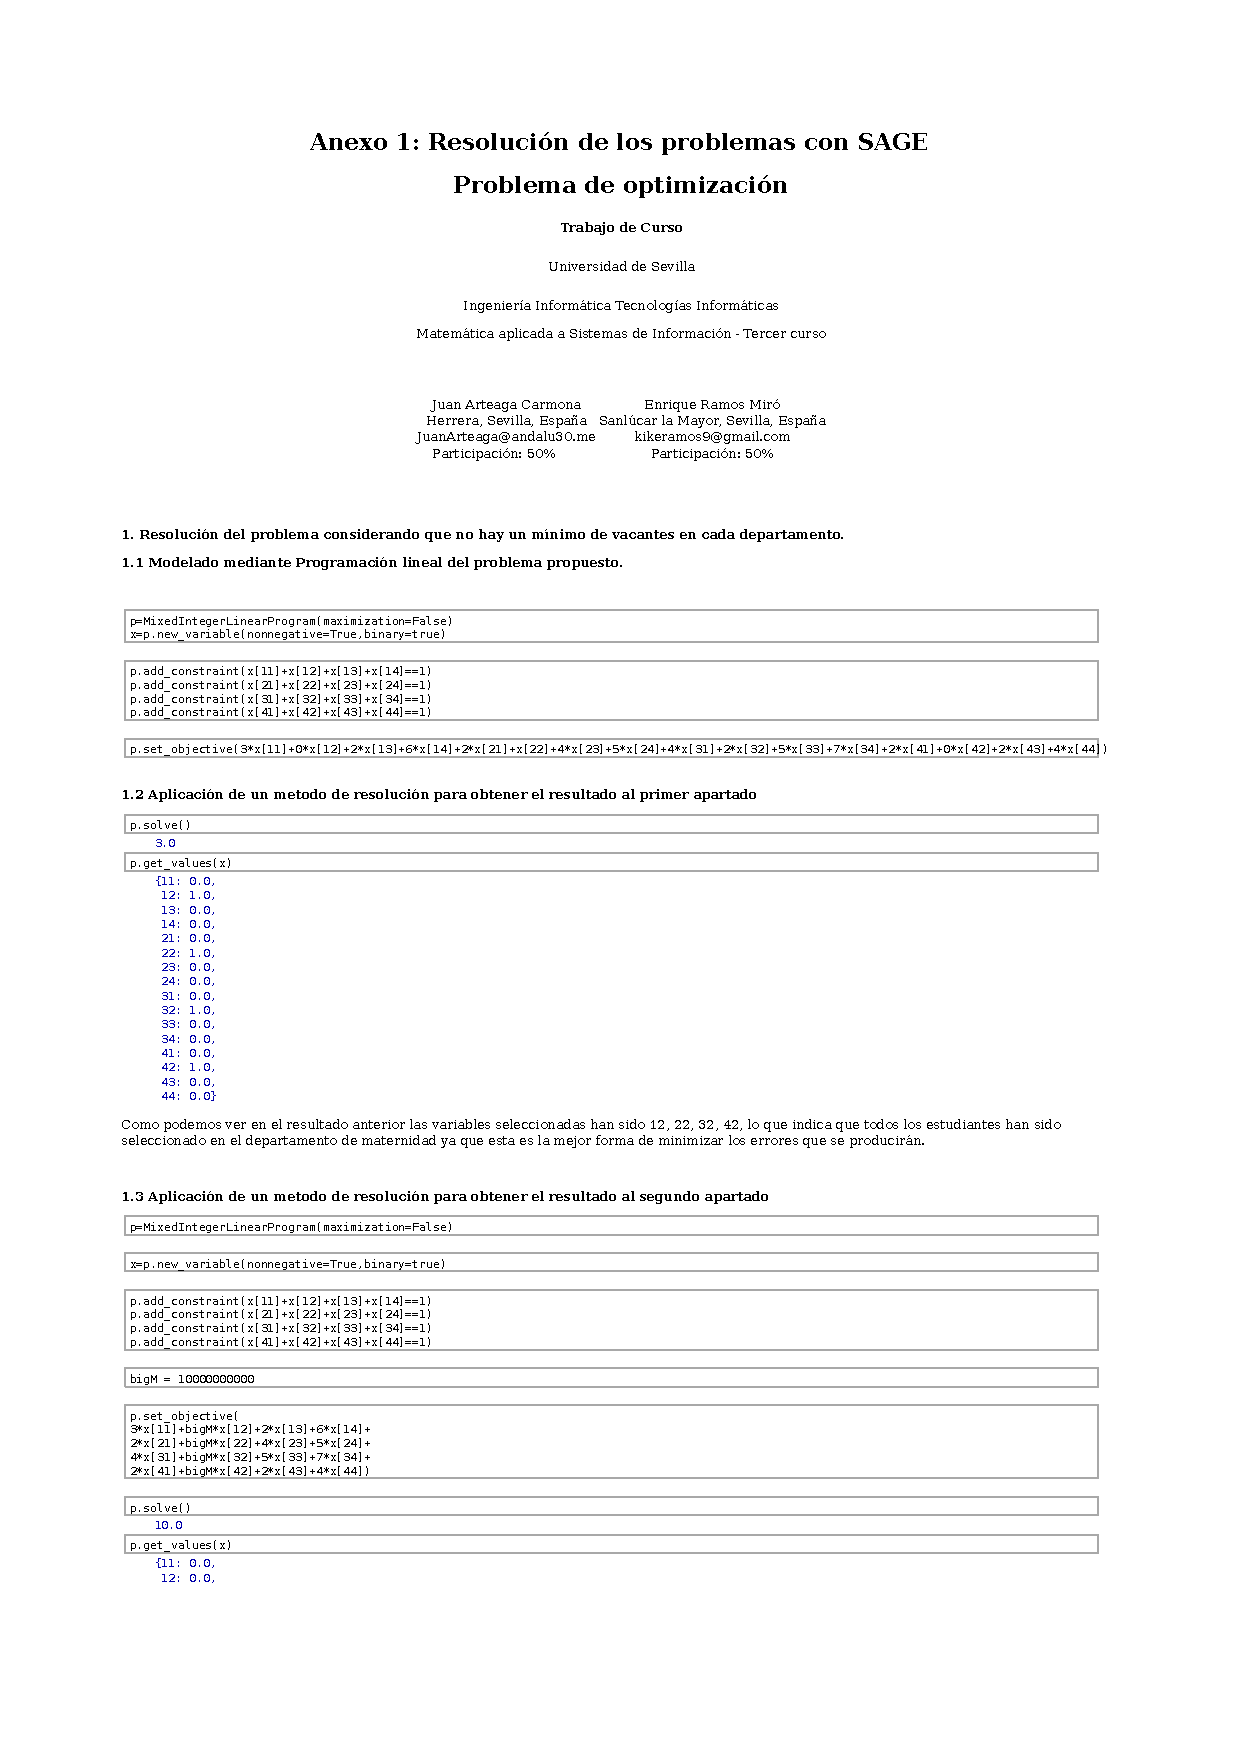
\includepdf[pages=-,frame,scale=0.95]{Anexo1.pdf}\label{pdf:anexo}




\end{document}
